\chapter{Installation}
These instructions are based on \miktex{} for \emph{Windows}.  Support for \emph{Linux} or other operating systems or \LaTeX{} installations is not available.

\section{Prerequisites}
\subsection{\LaTeX}
You can download a \emph{Windows} version as part of the \href{https://miktex.org}{\miktex{}} (www.miktex.org)\index{\miktex} project.

%\LaTeX{} is standard with most \emph{Linux} installations.

\subsection{Ghostscript and Ghostview}
Historically, it was required to install \emph{Ghostscript} and \emph{Ghostview}~\cite{ref:kopka1999a} in order to view \textcode{.eps} files and convert them to \textcode{.pdf}s.  However, it seems this requirement has been rendered obsolete by advances in \miktex{}.

It still can be useful to install these packages to allow viewing of \textcode{.eps} files.  \href{http://www.cs.wisc.edu/~ghost/}{\emph{Ghostscript} and \emph{Ghostview}}\index{Ghostscript}\index{Ghostview} can be downloaded at \href{http://www.cs.wisc.edu/~ghost/}{http://www.cs.wisc.edu/~ghost/}.
%\begin{plainlist}
%	\item \href{http://www.cs.wisc.edu/~ghost/}{http://www.cs.wisc.edu/~ghost/}
%\end{plainlist}

\subsection{\winedt}
A useful interface to \LaTeX{}/\miktex{} is provided by \href{https://www.winedt.com}{\winedt} (\href{www.winedt.com}{www.winedt.com}).  \winedt{} is highly customizable.  User interface features can be added to work with \lelatex{}.  For more information see the \emph{Installation Notes} in the repository \href{WinEdt Customizations}{https://github.com/lendres/WinEdt-Customizations}.


\section{LeLaTeX}
To completely install \lelatex{} takes several steps.  In the images that follow, \textcode{C:\tbs{}Custom Program Files\tbs{}LaTeX} is the folder the \lelatex{} library was downloaded to.

\begin{outline}
	\item Download the library from \href{https://github.com/lendres/LaTeX}{https://github.com/lendres/LaTeX} or your forked repository.
	\item Add \lelatex{} as a TEXMF directory.
	\begin{outline}
		\item Open the \miktex{} Console.
		\item Go to \emph{Settings$\rightarrow$Directories}
		\item Add the directory to as a TEXMF directory in the \miktex{} Console (see \figurename~\ref{fig:addastexmlroot}).
		\item Close the \miktex{} Console.
	\end{outline}
	\item Add the \textcode{Processing Support} directory to the \textcode{Path} environmental variable.
	\begin{outline}
		\item Open Windows System properties.
		\item Go to \emph{Advanced$\rightarrow$Environmental Variables} to open the environmental variables dialog box (see \figurename~\ref{fig:enironmentalvariables}).  You may need admin rights to edit the environmental variables.
		\item Edit the environmental variables and add the \textcode{./Processing Support} directory to the \textcode{Path} variable.
		\item Add the path the \textcode{.\tbs{}Processing Support\tbs{}} directory to the path.
	\end{outline}
	\item Install \emph{Strawberry Perl}
	\begin{outline}
		\item Download the installer from \href{https://strawberryperl.com/}{https://strawberryperl.com/}.
		\item Run the installer.
		\item Restart the computer.
	\end{outline}
\end{outline}


\begin{figure}
	\centering
	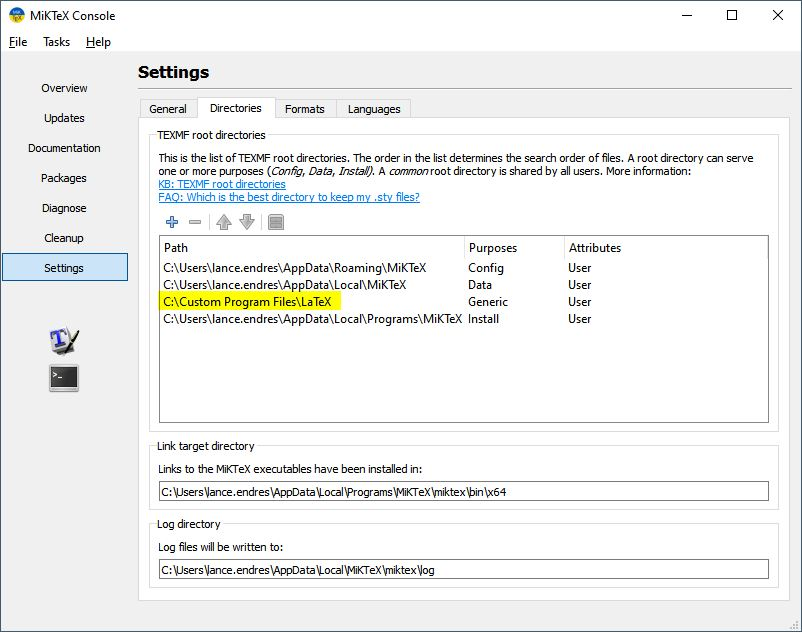
\includegraphics[height=3.0in]{addastexmlroot}
	\caption[Adding the library as a TEXMF root directory]{Adding the library as a TEXMF root directory.}
	\label{fig:addastexmlroot}
\end{figure}

\begin{figure}
	\centering
	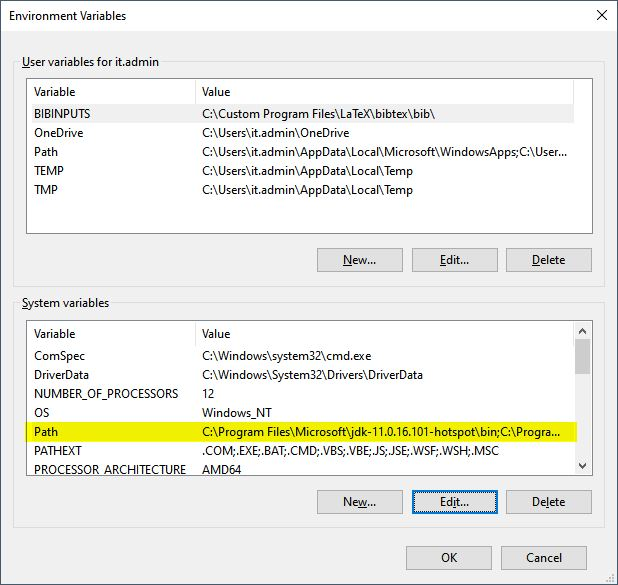
\includegraphics[height=3.0in]{enironmentalvariables}
	\caption[The environmental variable dialog box]{The environmental variable dialog box.}
	\label{fig:enironmentalvariables}
\end{figure}


\begin{figure}
	\centering
	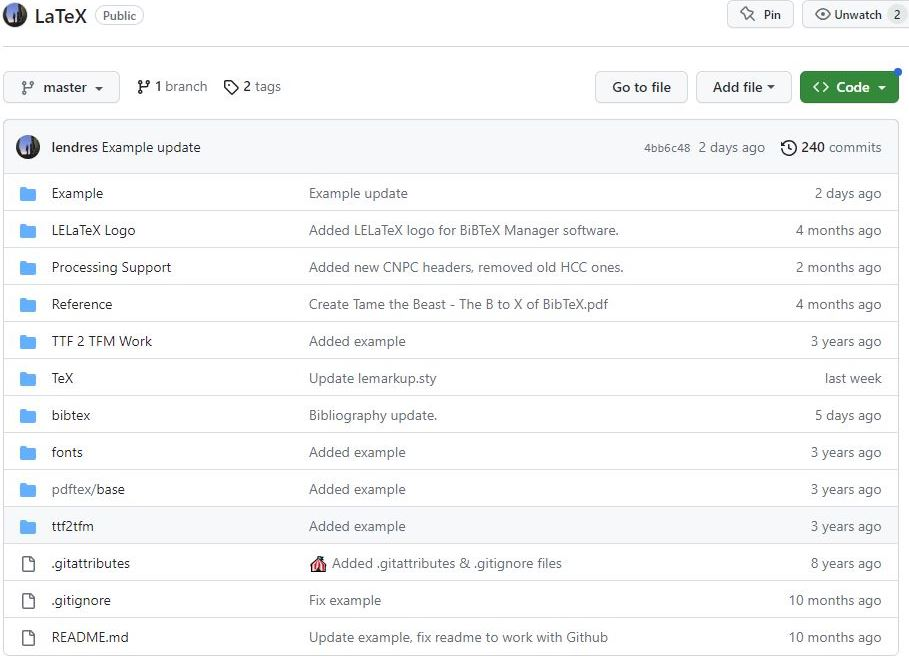
\includegraphics[height=2.5in]{githubwebsite}
	\caption[]{}
	\label{fig:githubwebsite}
\end{figure}

\begin{figure}
	\centering
	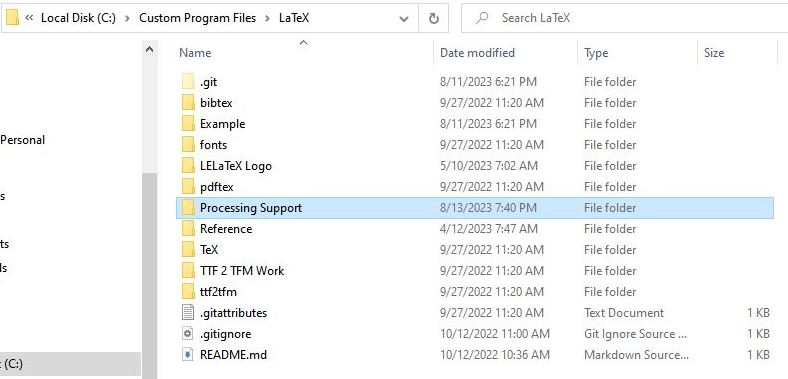
\includegraphics[height=3.0in]{latexroottexmfdirectory}
	\caption[]{}
	\label{fig:latexroottexmfdirectory}
\end{figure}


\begin{figure}
	\centering
	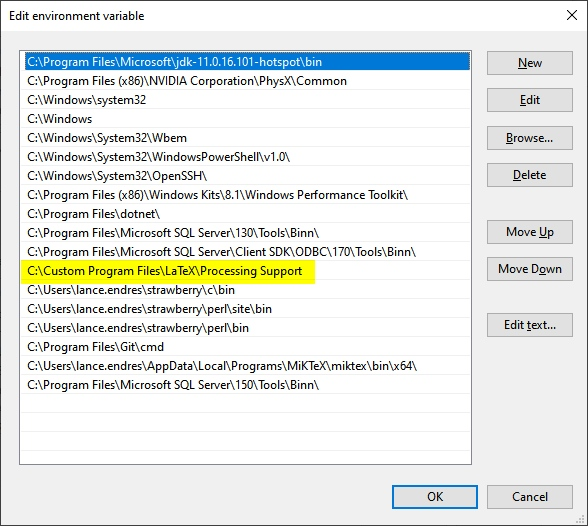
\includegraphics[height=3.0in]{pathenvironmentalvariable}
	\caption[]{}
	\label{fig:pathenvironmentalvariable}
\end{figure}

\begin{figure}
	\centering
	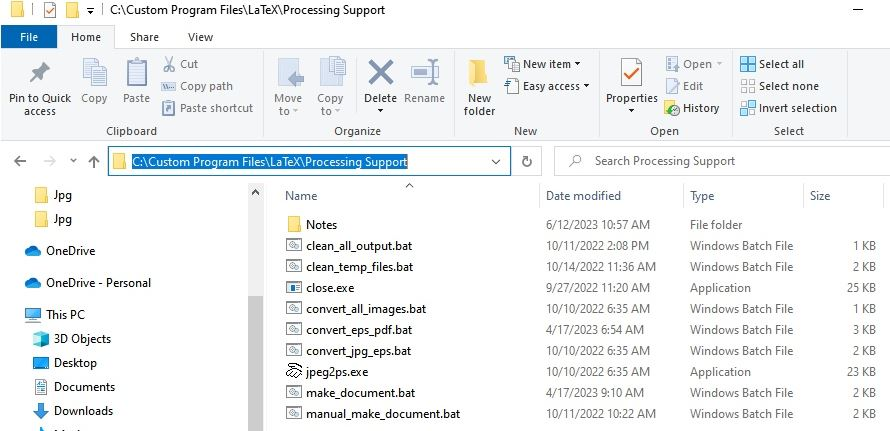
\includegraphics[height=3.0in]{processingsupportdirectory}
	\caption[]{}
	\label{fig:processingsupportdirectory}
\end{figure}

\begin{figure}
	\centering
	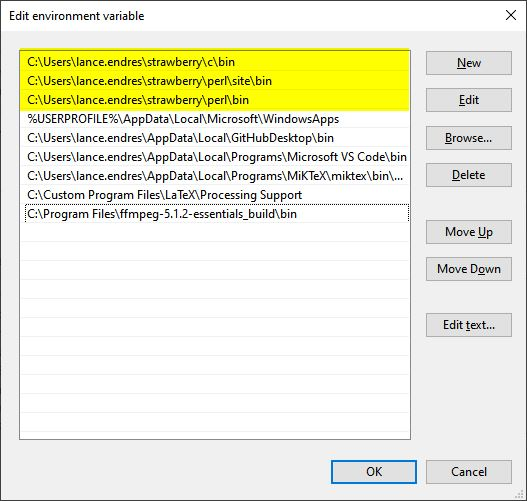
\includegraphics[height=3.0in]{strawberryperlpaths}
	\caption[]{}
	\label{fig:strawberryperlpaths}
\end{figure}
